\documentclass[conference]{IEEEtran}
\IEEEoverridecommandlockouts
% The preceding line is only needed to identify funding in the first footnote. If that is unneeded, please comment it out.
\usepackage[square]{natbib}
\setcitestyle{numbers}
\usepackage{amsmath,amssymb,amsfonts}
\usepackage{algorithmic}
\usepackage{graphicx}
\usepackage{textcomp}
\usepackage{cleveref}
\usepackage{xcolor}
\def\BibTeX{{\rm B\kern-.05em{\sc i\kern-.025em b}\kern-.08em
    T\kern-.1667em\lower.7ex\hbox{E}\kern-.125emX}}
\begin{document}

\title{Using CNN for letter recognition in images}

\author{\IEEEauthorblockN{Daniel Aaron Salwerowicz}
\IEEEauthorblockA{\textit{Institutt for datateknologi og beregningsorienterte ingeniørfag} \\
\textit{Arctic University of Norway, Narvik}\\
Narvik, Norway \\
dsa014@post.uit.no}
}

\maketitle

\begin{abstract}
In this report I describe my research related to developing CNN (Convolutional Neural Network) from scratch and then finding the best parameters to train it in recognizing letters in images. It shows how image is processed in between layers using my own implementation of them and then it shows what are the best parameters to use in such a network to develop best working model.
\end{abstract}

\begin{IEEEkeywords}
CNN, kernel, stride, letter recognition, object recognition, CIFAR-10
\end{IEEEkeywords}

\section{Introduction}
This research project revolved around finding the best parameters for learning a neural network to recognize letters in images. Parameters that I looked on were the pooling size, kernel and stride for convolutional layer, and dropout rate in between layers.

Firstly I focused on better understanding how CNNs work by implementing parts of it myself. After getting working model I ran my training set through it to see how images are transformed after being passed through each layer. Then I worked on training CNN to tell A and K letters apart from the rest of letters. Lastly I used CIFAR-10 data set to better train it with a huge data set so that I could get better results.

\section{Problem specification}
Main problem that I focused on was choosing right kernel and stride size for convolution layers as well as dropout between layers. 

To begin with I needed to get better understanding how CNNs work, I done that by implementing a few layers without using any standard libraries like Keras or Tensorflow. Each layer included a convolutional layer with various kernels, a rectifier that is a simple ReLU, and lastly max pooling. Convolution in a layer simply takes a matrix representing the image's colour values (from 0 to 1, inclusive) and  applies a kernel to it, starting in the top left corner moving to the right and down with a given kernel. Rectifier activates neuron based on the value put out by it, in the case of simple ReLU it is: $\text{ReLU}(x) = \text{max}(0,x)$. Pooling layer essentially downsizes the image by looking at a portion of a matrix, choosing the maximal or minimal value in that portion before moving along in the similar fashion to convolutional layer.

After that I used Keras and Tensorflow along with other standard libraries to train my CNN model in recognizing letter images.

Lastly I was tasked to used that knowledge and try to set up a simple CNN that would give satisfactory results in categorizing CIFAR-10 dataset.

\section{Methods applied}
When it comes to the implementation of convolution layer it was done simply by using NumPy's arrays to optimize operation time of my program. When an image is loaded and converted into a matrix it is simply iterated over and each part of it is multiplied piecewise with the kernel matrix and summed which is then put into the result matrix. this is done by utilizing NumPy functions sum and multiply that work much faster than conventional for loops would work. Code can be seen here: \verb|result[x, y] = sum(multiply(map, kernel))| where map is a portion of feature map that gets multiplied with kernel.

Pooling works in similar fashion where I iterate over feature map and choose the biggest element in the portion of it. ReLU itself is a mere line long where I create a lambda method that returns $x$ or $0$ depending on which one is bigger, vectorize this lambda and used vectorized method on the feature map.

To learn my model to recognize letters I used Keras and Tensorflow and their Sequential model with 3 convolutional layers LeakyReLU and MaxPooling in between them before flattening and condensing the result. I also used 4 dropout layers in between to avoid overfitting. Same techniques were used to categorize CIFAR-10 dataset.

\section{Results}
Results from my own implementation of CNN can be seen in \cref{fig:FirstPart}, as one can clearly see here the edges of letter are visibly enchanced while values for noise are brought down by a huge factor. This is shown by red-ish pixels around A before processing which show values between 0.9 to 1.0, which have been reduced to at most 0.05. Edges are emphasized since I am using an edge kernel in my convolutional layers, shown in \cref{eq:kernel}

\begin{equation}
\begin{bmatrix} 
-1 & -1 & -1 \\ 
-1 & 8 & -1 \\ 
-1 & -1 & -1
\end{bmatrix}
\label{eq:kernel}
\end{equation}

\begin{figure}[htbp]
  \centerline{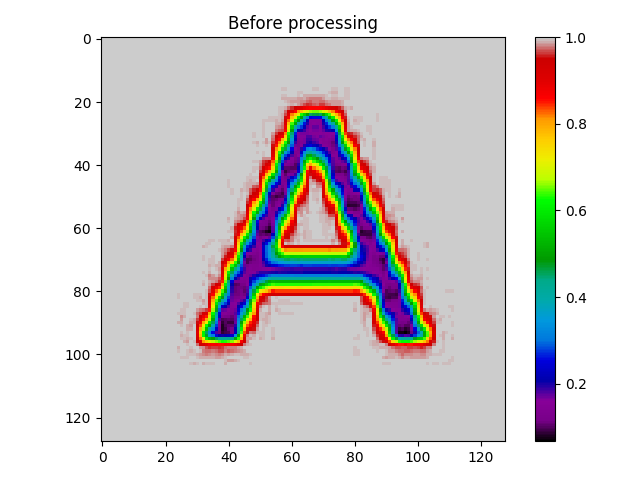
\includegraphics[width=.4\textwidth]{A_Zero_Layer}}
  \centerline{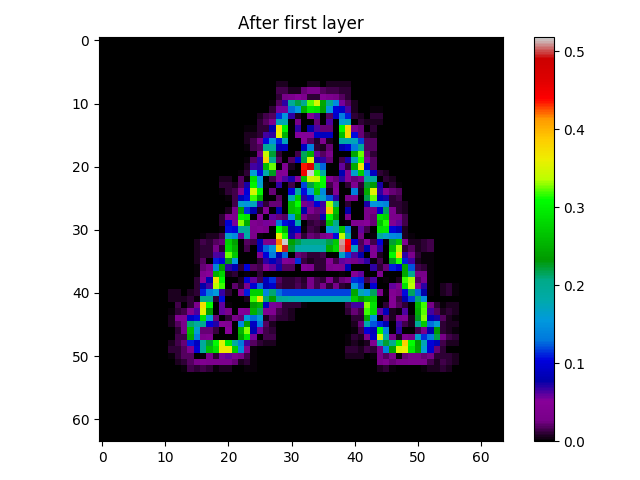
\includegraphics[width=.4\textwidth]{A_First_Layer}}
  \centerline{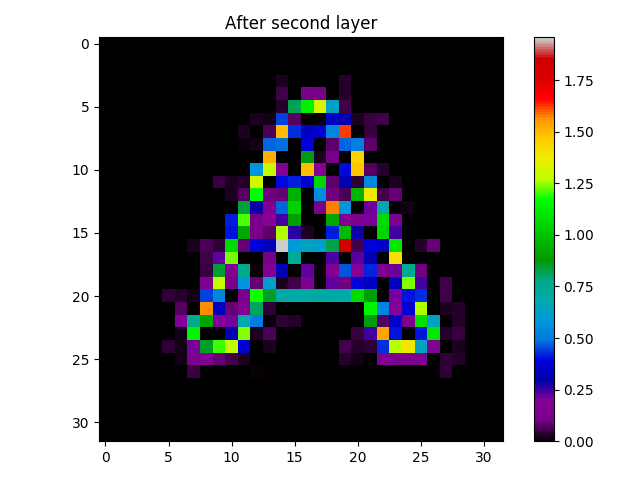
\includegraphics[width=.4\textwidth]{A_Second_Layer}}
\caption{Visualization of a matrix for letter A before and after it went through two layers of my CNN.}
\label{fig:FirstPart}
\end{figure}

Results for most of the letters are quite satisfactory, however since the sample size I have gotten was of really bad quality (noise from jpeg compression), not all letters look as good. Though I have managed to reduce it by sharpening the images.

Surprising thing happened when I tried to get my model to defferentiate between A and K. After many trials I ended up with a working model that was able to tell them apart $100\%$ of the time. However I needed to overtrain it in order to be able to do so. 

I have tried a lot of different kernel sizes, strides, as well as dropout values and to do it with and without pooling. None of them worked unless I overtrained my model. The values used are shown in \cref{tab:parametersLetters}. Dropout values were chosen based on research done in \cite{NIPS2013_4878}, and my own experimentation. 

As for what I did was run the tests for hundred epochs with various kernels, strides, and dropout various. Kernel sizes ranged from 3x3 to 5x5, strides went from 1x1 till 5x5, and dropout values tested were 0.2, 0.3, 0.4, 0.5, and 0.6.

Resulting test accuracy was $100\%$ with loss equal to $0.8\%$ percent. And graphs showing development of loss and accuracy can be seen in \cref{fig:LossAccLetters}.
\begin{table}[htbp]
  \centerline{
  \begin{tabular}{l l}
    Parameter    & Value \\
    Conv. kernel & 3x3   \\
    Conv. stride & 1x1   \\
    Pool. size   & 2x2   \\
    1st dropout  & 0.5   \\
    2nd dropout  & 0.4   \\
    3rd dropout  & 0.3   \\
    4th dropout  & 0.5   \\
    Epochs       & 420   \\\\
  \end{tabular}}
  \caption{Parameter values for recognizing letters in pictures.}
  \label{tab:parametersLetters}
\end{table}

\begin{figure}[htbp]
\centerline{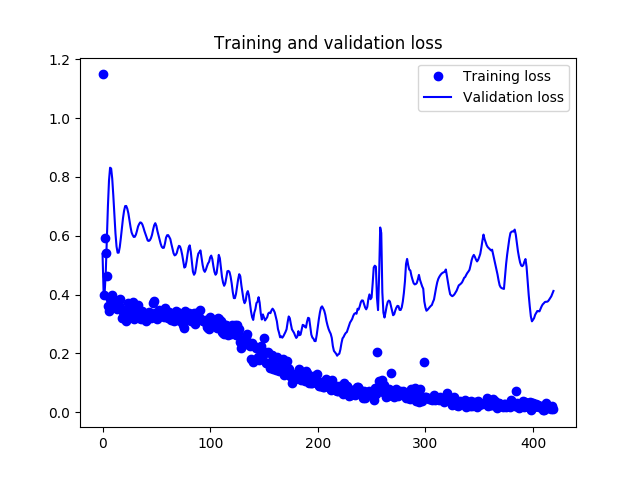
\includegraphics[width=.4\textwidth]{Letter_Loss}}
\centerline{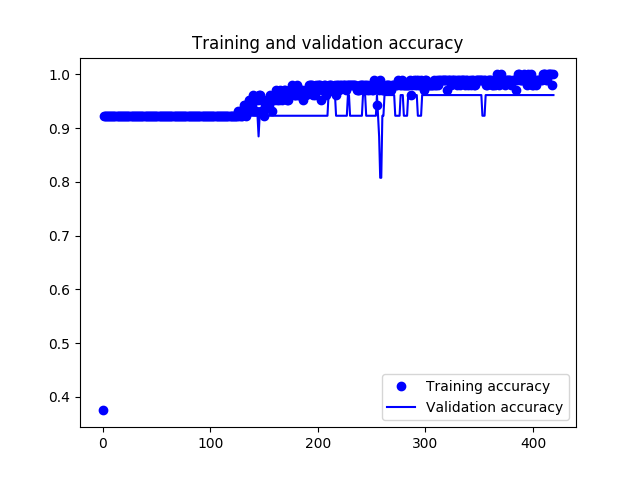
\includegraphics[width=.4\textwidth]{Letter_Accuracy}}
\caption{Loss and Accuracy graphs (respectively) for the training and validation data reached by my CNN on letters.}
\label{fig:LossAccLetters}
\end{figure}

As one can see from the graphs model started overfitting around epoch 200-220, wheras training accuracy went up after 150 epochs, while validation accuracy reached its peak around 300th epoch. It needs to be mentioned that because of the high dropout rate in first and last layer it is not a predictable model and it can sometimes end up with worse accuracy. Sometimes when I ran the training on this model I ended up with only $95\%$ accuracy as it couldn't recognize A, K, or both.

Lastly, results for the training on CIFAR-10 look much better as I don't overfit my model and they seem to coincide with research done by others who used simple CNNs \cite{DBLP:journals/corr/McDonnellV15}. I ended up with accuracy around $79\%$ and a loss of $62\%$. Although the loss value is quite high, it's similar to what others have achieved and the model itself is not overfitted. \Cref{tab:parametersCIFAR} shows values used in the final model.
\cref{fig:LossAccLetters}.
\begin{table}[htbp]
  \centerline{
    \begin{tabular}{l l}
      Parameter    & Value \\
      Conv. kernel & 3x3   \\
      Conv. stride & 1x1   \\
      Pool. size   & 2x2   \\
      1st dropout  & 0.5   \\
      2nd dropout  & 0.3   \\
      3rd dropout  & 0.5   \\
      4th dropout  & 0.3   \\
      Epochs       & 200   \\\\
  \end{tabular}}
  \caption{Parameter values for categorizing pictures in CIFAR-10 dataset.}
  \label{tab:parametersCIFAR}
\end{table}

It's worth mentioning that I have trained 128 models with kernel and stride sizes ranging from 1x1 to 10x10. The best was shown to be 3x3 kernel size with 1x1 dropout, whereas the worst one was and 8x8 kernel with stride of 1x1, it had a loss equal to $253\%$ and accuracy of $67\%$. \Cref{fig:LossAccCIFAR} show development of the model.

\begin{figure}[htbp]
  \centerline{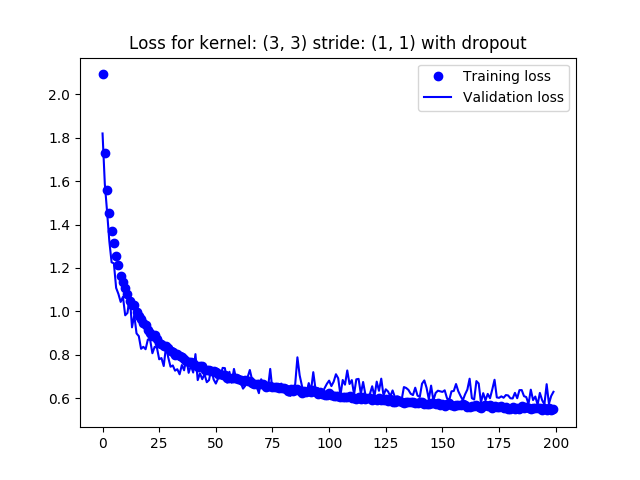
\includegraphics[width=.4\textwidth]{Best_Loss}}
  \centerline{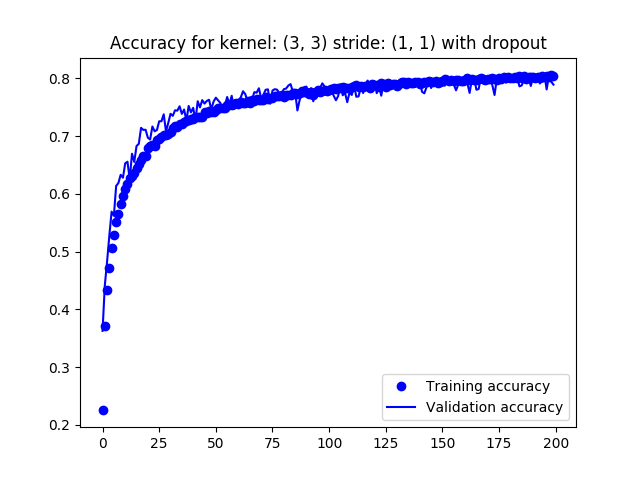
\includegraphics[width=.4\textwidth]{Best_Accuracy}}
  \caption{Loss and Accuracy graphs (respectively) for the training and validation data reached by my CNN on CIFAR-10 dataset.}
  \label{fig:LossAccCIFAR}
\end{figure}
\section{Discussion}
Overall I am very satisfied with my results. The results I got from my own convolution layers implementation were quite good given the dataset I had, and thanks to NumPy algorithms used it runs really fast.

The reason for need to overfit the model, in my opinion is based on relatively small dataset I have used in training my model and the bad quality of said set. A lot of pictures had were really bad in quality and low-res. I believe that if I had a bigger dataset like like MNIST I could achieve better results, much faster too.

Another thing that is worth giving a shot would be to add data augmentation to my training in the form of scaling, rotating, flipping, translating, etc. the data set. This could possibly give better results as I could artificially increase the data set this way. There are tools for this both in Keras and Tensorflow libraries.

When it comes to CIFAR-10 dataset I have noticed that my model struggles a lot with accurately categorizing pictures in the first class (Aeroplanes). It only achieved accuracy of around $43\%$ whereas the other 9 classes had accuracy scores raging from $77-92\%$. My explanation for it is the fact that a images in this set are very different from eachother and it's hard to distinguish them from others (I myself struggled to see the aeroplanes in them).

Overall I am content with my results and I have learned a lot along the way. I also believe that research I have done, with different kernel sizes and other parameters have given me insight and better intuition in choosing good values for a given task.

My work has of course a lot of room for further improvement, like aforementioned data augmentation and maybe adding of another layers to the model to further improve its results.


\section*{Acknowledgments}
I would like to thank Christopher Kragebøl Hagerup, Kent Arne Larsen, Hans Victor Andersson Lindbäck, and Olav Kjartan Larseng for helping me underway. We brainstormed a lot of ideas on how to solve this problem, and I worked a lot together with Christopher on the first part of this project.

\bibliographystyle{apalike}
\bibliography{Bibliography}

\end{document}
